\chapter{Hardware Development}

One of the cornerstones of our team's Concept of Operations for the SubT Challenge was modular autonomy. That is, we wanted to develop a series of modules which could be composed and rapidly reconfigured to suit the task at hand. The use of individual modules would also allow for components to be replaced or upgraded as necessary. For example, each of our ground robots had 4 drive modules, each consisting of a wheel, motor, gearbox, and a separate electronics module. The drive modules could be replaced or upgraded as necessary, such as in the case of a gearbox failing or the selection of different desired torque profiles. Similarly, we wanted to develop modular sensing and compute payloads which could be transferred across different robots, including in between ground and aerial robots, and which would be capable of performing all of the robot's high level autonomy functions.

Early indication that our approach should be feasible came as the result of using a prototype state estimation payload ("Blue Payload") similar to the Kaarta Traak \cite{kaarta_traak}. The payload was relatively small, self-contained, and could be easily transferred between robots (see Figure \ref{blue payload robots}). We simply had to mount the payload to the robot, apply power, and connect to the robot's internal network, and all of the payload's autonomy functions would be enabled. Overall, we found the Blue Payload quite simple to integrate, and wanted our future payloads to be similar in this regard. Inspired by the Blue Payload, and keeping the SubT Challenge requirements and timeline in mind, we came up with a list of some design goals and desired capabilities for our first payload ("Mk 0"), sorted by priority:

\begin{description}
	\item[Self-contained] All of the sensing and computation for the high level autonomy features should happen inside the payload itself. Ideally, the payload would only be supplied power and a network connection, just like the Blue Payload, and would output autonomy goals (such as waypoints) and information (such as robot state, maps, and artifact locations) to be relayed to the human supervisor at the base station.
	\item[Rapid Development] From the beginning of the competition (September 2018) to the first qualification deadline (December 2018), we had a little under 3 months to develop our first payload. This meant that, wherever possible, we should prefer designs that relied on existing expertise, such as the use of familiar components and sensors, and preferring in-house manufacturing capabilities with short lead times.
	\item[Environmentally Robust] We expected the field environments for the SubT competition to be somewhat hostile to the sensors. Specifically, we were told that "dust, fog, mist, water, and smoke are within scope" \cite{tunnel_rules}, and we wanted our payload to be reasonably protected against these elements, within reason. Additionally, the payload needed to be robust to the mechanical loading it would be subject to as a result of the rough terrain.
	\item[Weight Sensitivity] Similar to the Blue Payload, we wanted our new payload to be light enough to be carried by one of our aerial robots (as in Figure \ref{d1 blue payload}), or a smaller ground robot (as in Figure \ref{joeybot blue payload}) in addition to larger robots (as in Figure \ref{r1 blue payload}).
	\item[Low Cost] While there aren't specific restrictions on the maximum cost of our robot, DARPA was interested in identifying cost effective solutions for the SubT Challenge. Minimizing cost is also useful as a design goal as we intended to build multiple copies of the payload for our various robots, as well as to have spares.
\end{description}

\begin{figure}
	\centering
	\begin{subfigure}{0.3\textwidth}
		\includegraphics[width=\textwidth]{blue_payload_joeybot.png}
		\caption{Joeybot with Blue Payload}
		\label{joeybot blue payload}
	\end{subfigure}		
	\hfill
	\begin{subfigure}{0.3\textwidth}
		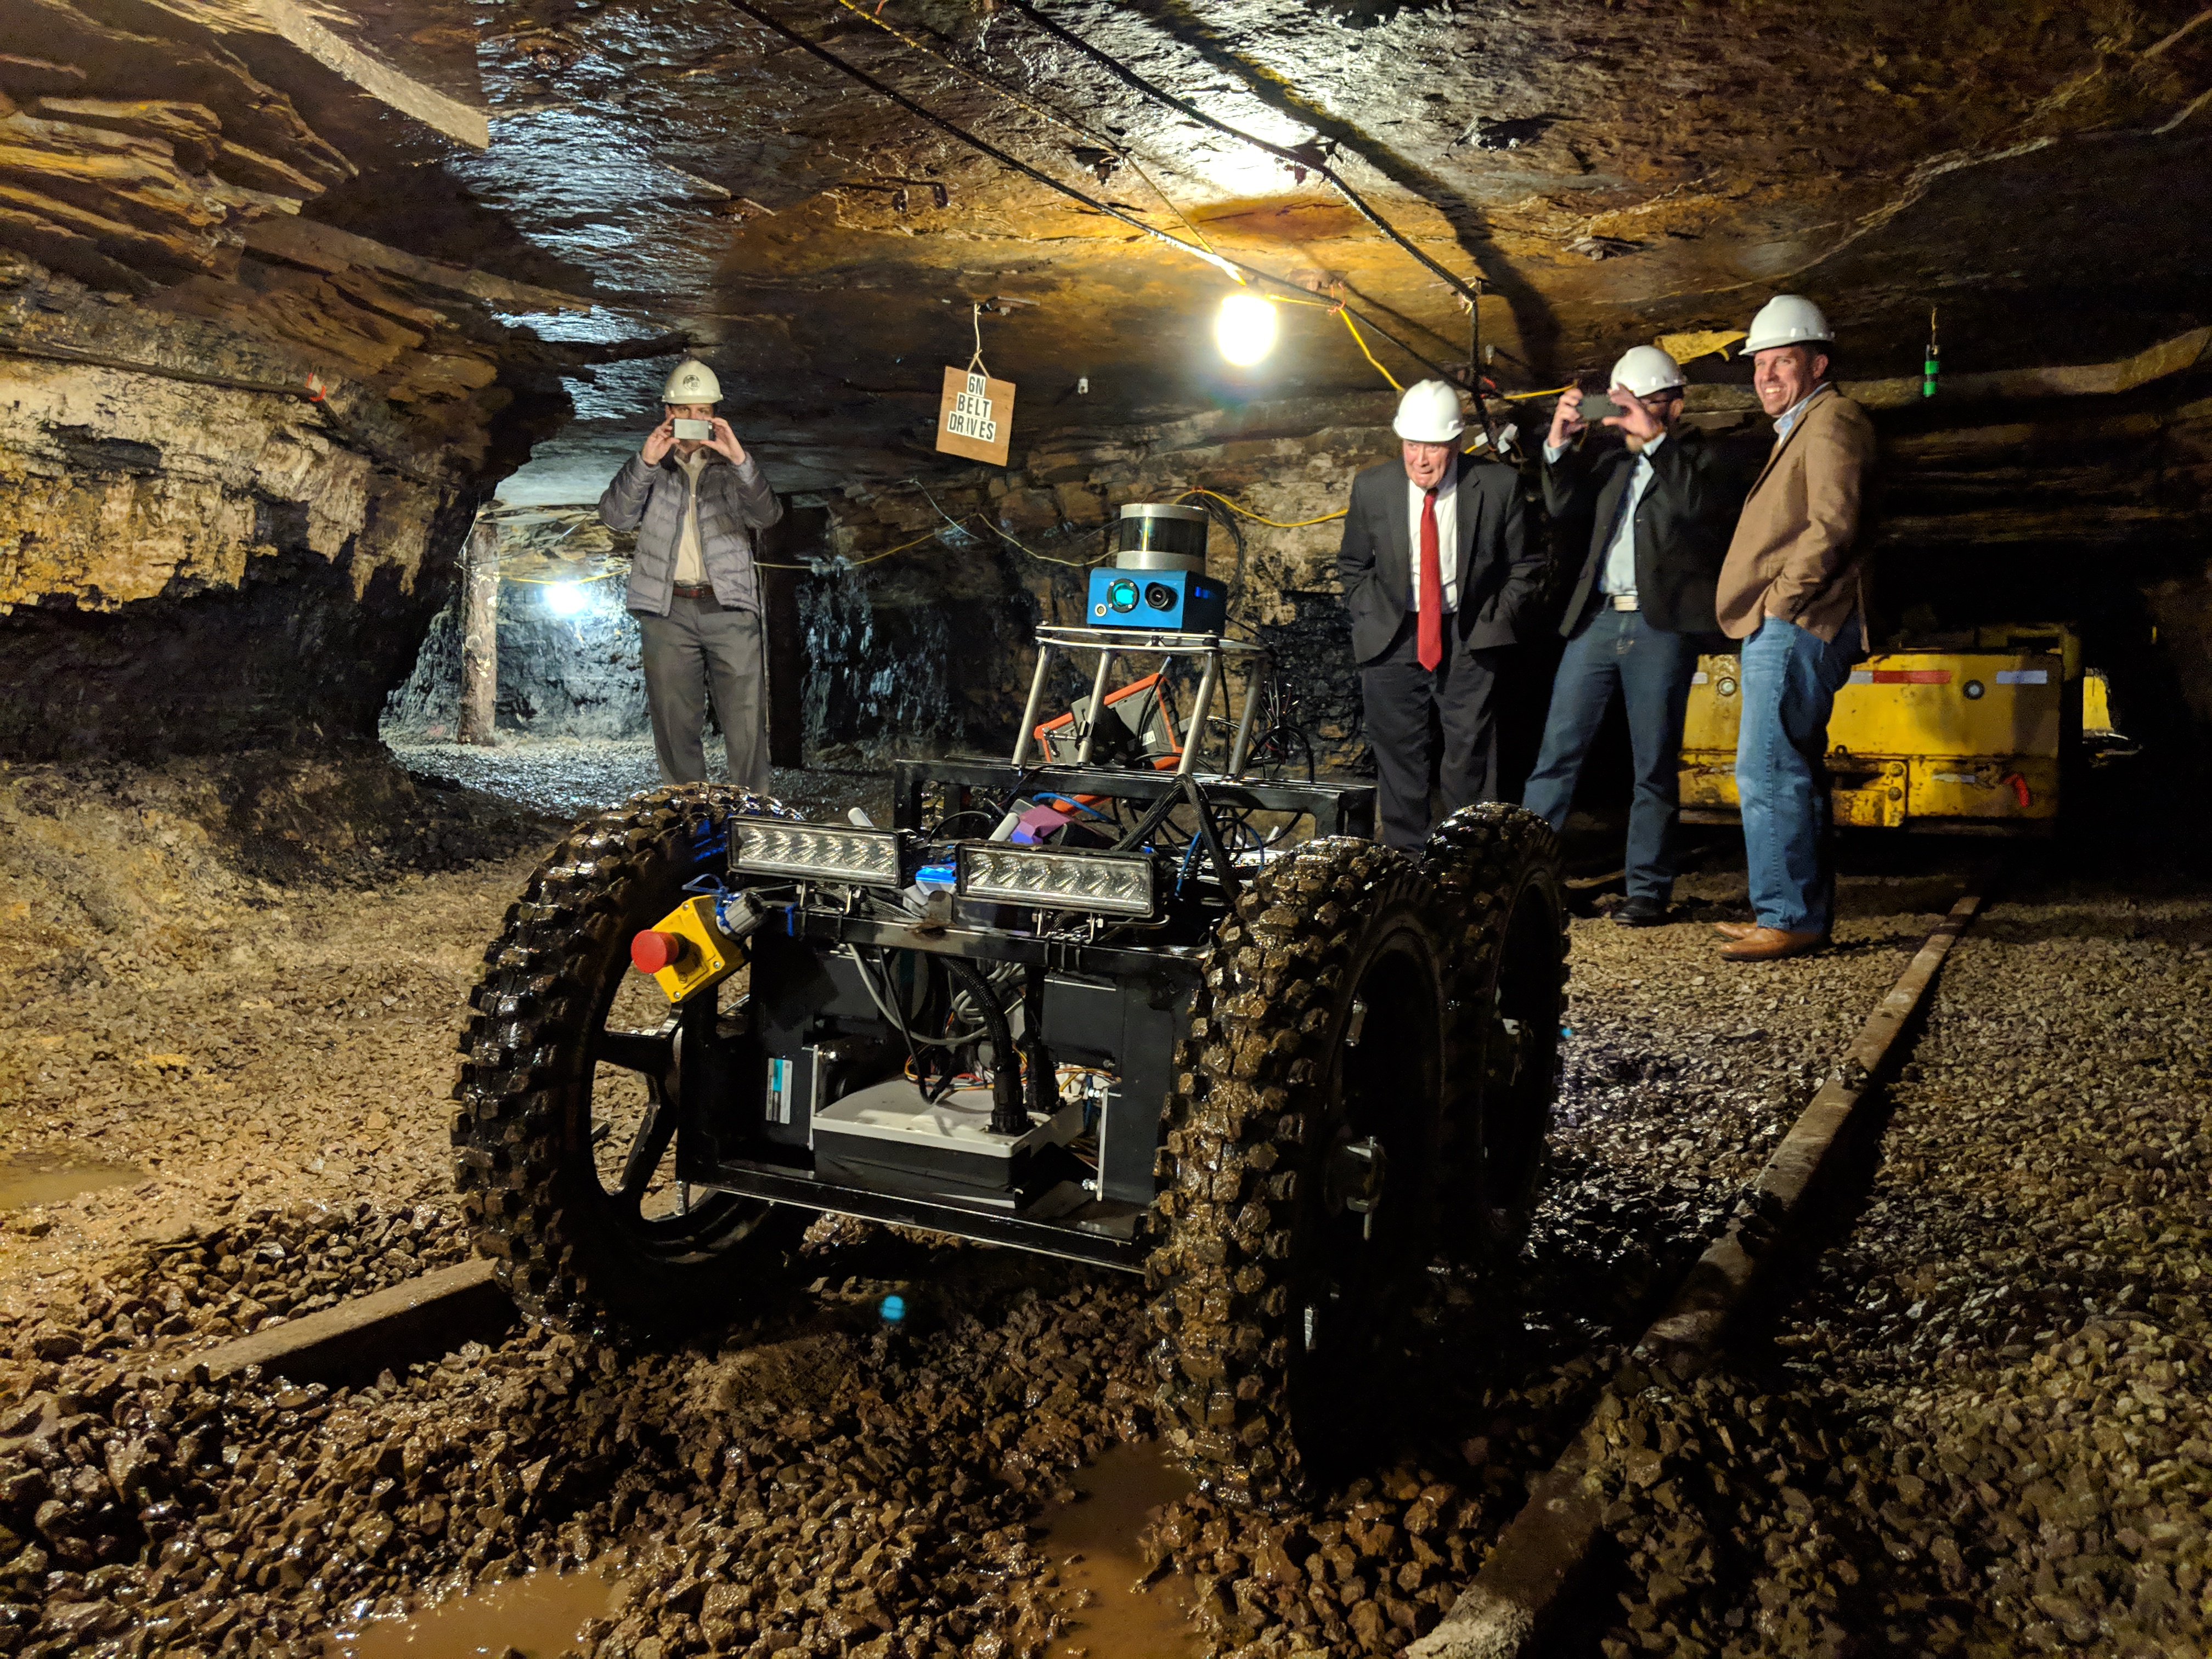
\includegraphics[width=\textwidth]{r1_with_blue_payload.jpg}
		\caption{R1 with Blue Payload}
		\label{r1 blue payload}		
	\end{subfigure}
	\hfill
	\begin{subfigure}{0.3\textwidth}
		\includegraphics[width=\textwidth]{drone_with_blue_payload.png}
		\caption{D1 with Blue Payload}
		\label{d1 blue payload}
	\end{subfigure}	
	\caption{Robots with initial modular payload ("Blue Payload")}
	\label{blue payload robots}
\end{figure}

\section{Mk. 0 Component Selection}

\subsection{Computer(s)}

In order to select the computer(s) to be used inside Mk. 0, it was important for us to figure out the tasks that the payload would need to perform. While we wouldn't be able to know exactly how many resources each of the tasks would consume, prior experience could help us determine some rough approximations. The main tasks for the payload would be the following:

\begin{enumerate}
	\item State estimation
	\item Path planning and navigation
	\item Object detection and localization
\end{enumerate}

For state estimation, we knew that we would be using LOAM \cite{zhang2014loam}, which was written by Ji Zhang (one of our team members), and is the current state of the art for SLAM. We knew that LOAM ran well on the Blue Payload, which uses an Intel NUC with an Intel Core i7 processor internally. The path planning and navigation stack was being actively developed and ran on the second computer on Joeybot (see Figure \ref{joeybot blue payload}), which was a mid-range industrial-grade PC from Logic Supply. Though the Logic Supply computer was also using an Intel Core i7 processor, the processor itself was underclocked to reduce heat output. Profiling indicated that it should be possible to run the path planning and navigation stack on the NUC being used to run LOAM, especially given the underclocked processor in the Logic Supply computer. This factor, along with various team members' familiarity with the NUC family of products, marked the Intel NUC as a strong contender for use in our payload. Specifically, we considered the NUC8i7BEB, which the best (with regards to CPU) available NUC board at the time.

Working under the assumption that we'd use an Intel NUC inside the payload, the question of running the object detection and localization stack still remained. While it wasn't yet clear what our object detection strategy would be, the use of convolutional neural networks in advancing the state of the art for object detection suggested that they would be a component of our approach. To efficiently run convolutional neural networks, a few hardware platforms were considered. We attempted to find a platform which we thought could run multiple neural networks in parallel, at relatively high frequencies (10+ Hz). We considered the following options:

\begin{enumerate}
	\item Intel Movidius Neural Compute Stick
	\item NUC8i7BEB integrated GPU (Intel Iris Plus Graphics 655)
	\item Nvidia Jetson TX2
	\item Nvidia Jetson AGX Xavier
\end{enumerate}

Of the available options, the Nvidia Jetson AGX Xavier ("Xavier") offered the highest inference performance due to its many CUDA cores, as well as its specialized Tensor Cores and Deep Learning Accelerators. Combined, the Xavier was capable of performing more than an order of magnitude more FLOPS than the other platforms. As we were unsure of the exact requirements of our object detection system at the time, we chose to overprovision, and thus the available FLOPS became the deciding factor. The Xavier emerged as the clear winner for our GPU selection inside the Mk. 0 payload. At this stage, it was also decided to commit to using the NUC8i7BEB inside Mk. 0. In an attempt to simplify the system, we briefly considered attempting to run the entire autonomy stack on a single Xavier, rather than split between a NUC and an Xavier. However, we felt that the slower ARM cores on the Xavier would not be able to handle the combined autonomy stack, and thus decided to continue using both computers inside the Mk. 0 payload.

After the completion of the Mk. 0 payload, we performed some experiments to see if our earlier hypothesis about the Xavier being unable to handle the entire autonomy stack was correct. Profiling of the NUC revealed that LOAM was one of the heaviest processes, consuming nearly 100\% of a single core in some circumstances, and smaller portions of other cores. Thus, we decided to attempt to run LOAM on the Xavier first. For our benchmarking, we set up an Xavier Developer Kit in MAX-N mode after having disabled the frequency governors with the provided jetson\_clocks.sh script. This mode enables all of the processors in the Xavier, and pins them at their highest frequency. We attempted to run LOAM on pre-recorded data in a few different configurations, varying a parameter to adjust downsampling of the input point clouds to reduce the scan alignment cost. Figure \ref{loam_xavier} shows a visualization of the results.

\begin{figure}
	\centering
	\begin{subfigure}{0.3\textwidth}
		\includegraphics[width=\textwidth]{tour_ed_mine_1-00.png}
		\caption{100\% Point Cloud Scaling}
		\label{loam_xavier_100}
	\end{subfigure}		
	\hfill
	\begin{subfigure}{0.3\textwidth}
		\includegraphics[width=\textwidth]{tour_ed_mine_1-00_1-25s.png}
		\caption{75\% Point Cloud Scaling}
		\label{loam_xavier_75}		
	\end{subfigure}
	\hfill
	\begin{subfigure}{0.3\textwidth}
		\includegraphics[width=\textwidth]{tour_ed_mine_1-00_1-50s.png}
		\caption{50\% Point Cloud Scaling}
		\label{loam_xavier_50}
	\end{subfigure}	
	\caption{Visualization of LOAM running on an Xavier with different downsampling parameters, using pre-recorded data collected at the Tour-Ed Mine in Tarentum, PA.}
	\label{loam_xavier}
\end{figure}

In Figure \ref{loam_xavier_100}, the same configuration as the NUC on Mk. 0 was used. Severe misalignment is visible - the lower tunnel does not align correctly, and a secondary "ghost" tunnel is created. In Figure \ref{loam_xavier_75}, 75\% of the laser scanner's points are kept. This does result in better alignment, though the images of two tunnels are still clearly visible in the figure. Finally, in Figure \ref{loam_xavier_50}, only 50\% of the laser scanner's points are kept. In this environment, the point cloud alignment is successful, suggesting that the state estimate did not drift significantly. However, the requisite 50\% downsampling was deemed to be too significant, as it presented a high risk of misalginment under harsh motions or in feature-bare environments due to the low density of points. This experiment confirmed our initial hypothesis that, without significant optimization, our current autonomy stack would be unable to run on a single Xavier.

\subsection{Sensor(s)}
\subsection{Miscellaneous}

\begin{enumerate}
	\item Computers (for both object detection and SLAM)
	\item Sensing (both for SLAM and object detection), as well as sensor placement 
	\item sensor synchronization (maybe not its own bullet?)
	\item power management / distribution (everything in the box should be powered by a single cable)
	\item connectors (internal and external) (including debugging)
	\item heat dissipation (more of a mechanical problem)
	\item mounting
\end{enumerate}